\chapter{Implementation}
%\textit{I give the overview of the project repository. I move on to explain the  }
%
%\section{Repository Overview}
%
%\dirtree{%
%	.1 P4-NetFPGA.
%		.2 project.
%			.3 simple\_sume\_switch.
%				.4 hw.
%					.5 hdl.
%						.6 nf\_datapath.v*.
%				.4 test.
%					.5 sim\_switch\_default.
%						.6 run.py*.
%			.3 src.
%				.4 tcp\_retransmit.p4*.
%				.4 commands.txt*.
%			.3 testdata.
%				.4 gen\_testdata.py*.
%				.4 digest\_data.py*.
%				.4 sss\_sdnet\_tuples.py*.
%			.3 templates.
%				.4 externs.
%					.5 <externs\_type>.
%						.6 hdl.
%							.7 <externs\_type>\_template.v*.
%		.2 lib.
%			.3 hw.
%				.4 contrib.
%					.5 cores.
%						.6 sss\_cache\_queues\_v1\_0\_0*.
%				.4 std.
%					.5 cores.
%						.6 output\_arbiter\_v1\_0\_0*.
%}

\section{Software Implementation}
	\subsection{The Parser}
Parsers are functions that are responsible for extracting headers out of an incoming packet, written in a state machine style. The following code sequence defines our parser with a \texttt{start} state:

{\renewcommand{\baselinestretch}{0.8}\small
	\begin{verbatim}
    // Parser Implementation
    @Xilinx_MaxPacketRegion(8192)
    parser TopParser(packet_in b, 
                    out Parsed_packet p, 
                    out user_metadata_t user_metadata,
                    out digest_data_t digest_data,
                    inout sume_metadata_t sume_metadata) {
      state start {
        b.extract(p.ethernet);
        user_metadata.unused = 0;
        digest_data.unused = 0;
        digest_data.flow_id = 0;
        digest_data.tuser = 0;
        transition select(p.ethernet.etherType) {
          IPV4_TYPE: parse_ipv4;
          default: reject;
        } 
      }   
    }
	\end{verbatim}
}
where \texttt{@Xilinx\_MaxPacketRegion} is Xilinx P4-SDNet's additional annotation for parser/deparser that declares the largest packet size (in bits) the parser/deparser needs to support.

\begin{figure}[h]
	\centering
	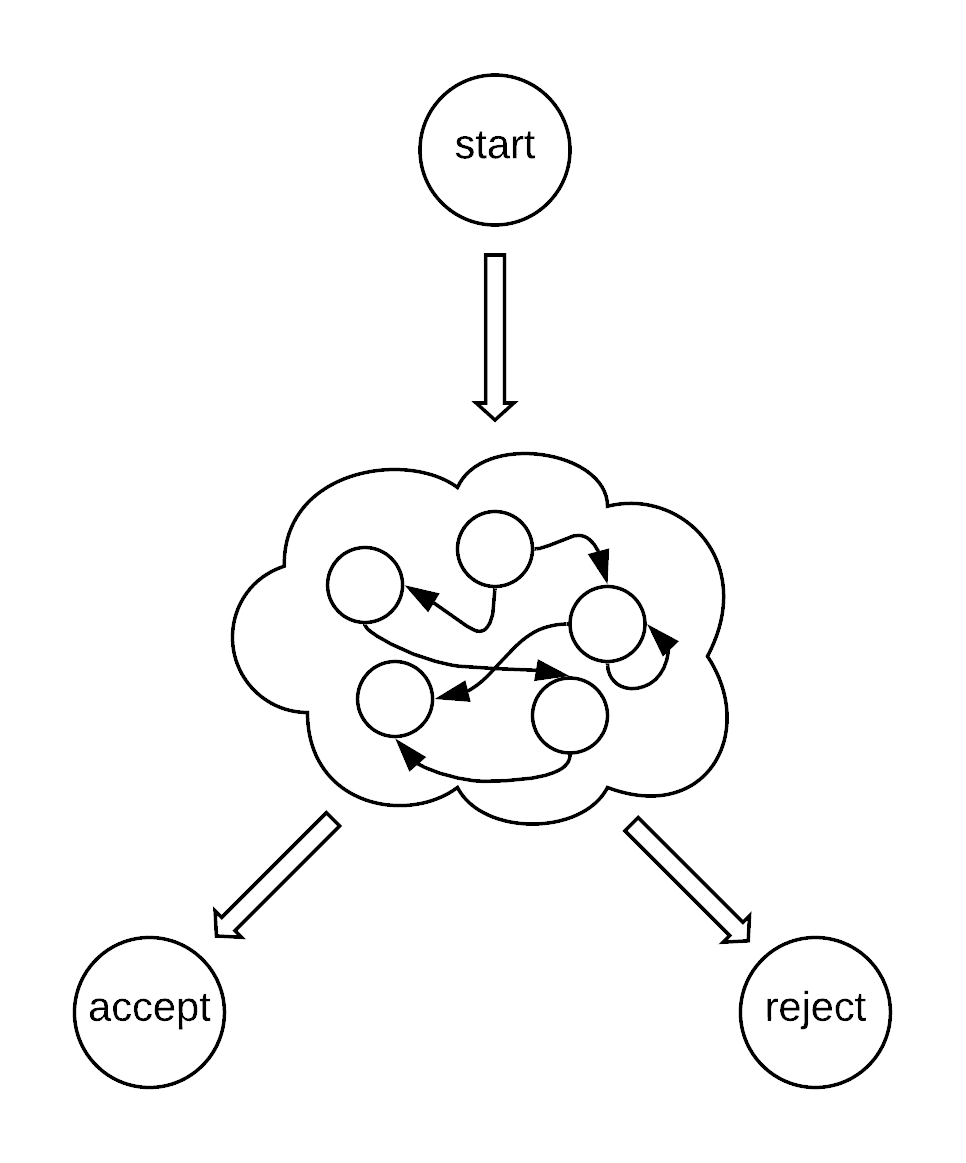
\includegraphics[width=0.4\textwidth]{general-fsm.png}
	\caption{Parser general FSM structure.}
	\label{general-fsm}
\end{figure}
 
Figure \ref{general-fsm} illustrates the general structure of a parser state machine, which includes three predefined states: 
\begin{itemize}
	\item \texttt{start} -- the start state.
	\item \texttt{accept} -- indicating successful parsing.
	\item \texttt{reject} -- indicating a parsing failure.
\end{itemize}
and other internal states that may be defined by the user. Parsers always start in the \texttt{start} state, execute one or more statements, then make a transition to the next state until reaching either the \texttt{accept} or \texttt{reject} states, which are distinct from the user-defined states and are logically outside of the parser. 

An architecture must specify the behaviour when the \texttt{accept} and \texttt{reject} states are reached. For example, an architecture may specify that all packets reaching the \texttt{reject} state are dropped without further processing. Alternatively, it may specify that such packets are passed to the next block after the parser, with intrinsic metadata indicating that the parser reached the \texttt{reject} state, along with the error recorded. The SimpleSumeSwitch architecture adopts the former.

\begin{figure}[h]
	\centering
	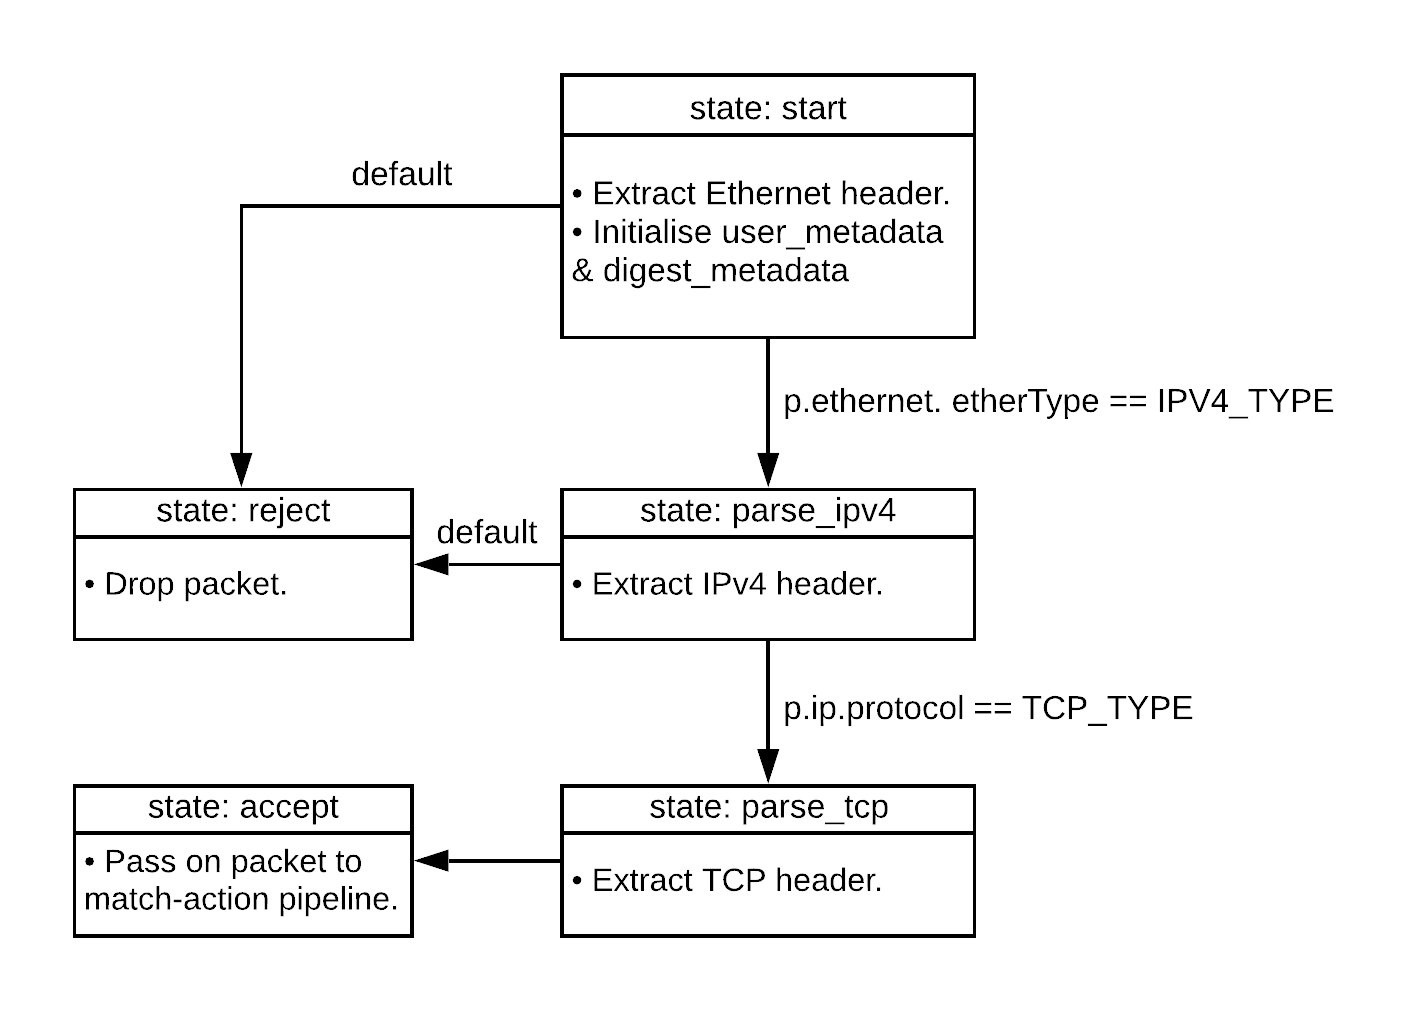
\includegraphics[width=0.8\textwidth]{design-fsm.png}
	\caption{The FSM of the design.}
	\label{design-fsm}
\end{figure}

Figure \ref{design-fsm} describes the FSM structure of our parser, in which I defined two additional states \texttt{parse\_ipv4} and \texttt{parse\_tcp}:

\begin{figure}[!h]
	\begin{minipage}{.48\textwidth}
		{\renewcommand{\baselinestretch}{0.8}\small
		\begin{verbatim}
		state parse_ipv4 {
		  b.extract(p.ip);
		  transition select(p.ip.protocol) {
		    TCP_TYPE: parse_tcp;
		    default: reject;
		  }
		}
		\end{verbatim}
		}
 		\caption{The definition of \texttt{parse\_ipv4} state.}
	\end{minipage}
	\hfill
	\begin{minipage}{.48\textwidth}
		{\renewcommand{\baselinestretch}{0.8}\small
		\begin{verbatim}
		state parse_tcp {
		  b.extract(p.tcp);
		  transition accept;
		}
		    
		    
		    
		\end{verbatim}
		}	
		\caption{The definition of \texttt{parse\_tcp} state.}
	\end{minipage}
\end{figure}

The P4 \texttt{select} statement is used to branch in a parser. It is similar to \texttt{case} statement in C or Java, but without ``fall-through behaviour''---i.e., \texttt{break} statements are not needed. Here, our parser first uses the \verb|packet_in| object's \texttt{extract} method to fill out the fields of the Ethernet header. It also initialises the values of the \verb|user_metadata|'s field \verb|digest_data|'s fields to 0. It then transitions to either the \verb|parse_ipv4| state or the \texttt{reject} state based on the value of the Ethernet header’s \texttt{etherType} field. In the \texttt{parse\_ipv4} state, the parser extracts the packet's IPv4 header, looks at its \texttt{protocol} field and transitions to the \texttt{parse\_tcp} state only if it is \texttt{TCP\_TYPE} which is defined to be 6. Otherwise, the packet is rejected. Finally, in the \texttt{parse\_tcp} state, the parser simply extracts the TCP header and then transitions to the \texttt{accept} state, where the packet will be passed to the match-action pipeline. A \texttt{parse\_ethernet} state could be defined similarly to \verb|parse_ipv4| and \verb|parse_tcp|, but I decided to include the parsing of the Ethernet header within the \texttt{start} state, together with initialising the metadata, for simplicity.
		
	\subsection{The Match-Action Pipeline}
A match-action pipeline is a control block where the match-action packet processing logic is implemented. A match-action pipeline uses tables, actions, and imperative code (indicated by the \textbf{\texttt{control}} keyword) to manipulate input headers and metadata. This match-action processing model was originally introduced as the core around which the OpenFlow model for SDN was built \cite{}. Our match-action pipeline can be defined by the following code sequence:

{\renewcommand{\baselinestretch}{0.8}\small
	\begin{verbatim}
    // Match-action pipeline
    control TopPipe(inout Parsed_packet p,
                  inout sume_metadata_t sume_metadata, 
                  inout digest_data_t digest_data, 
                  inout user_metadata_t user_metadata) {
      /** actions **/
      /** tables **/
      /** logic **/          
    }
	\end{verbatim}
}

This pipeline receives four inputs: the parsed packet \texttt{p}, the SUME metadata, the digest data and the user metadata. The direction \texttt{inout} indicates that the parameters are both an input and an output. Thus, their values, including the fields in the headers of packet \texttt{p}, can be modified. Nonetheless, the user metadata was not used in this design.

\begin{figure}[!ht]
	\centering
	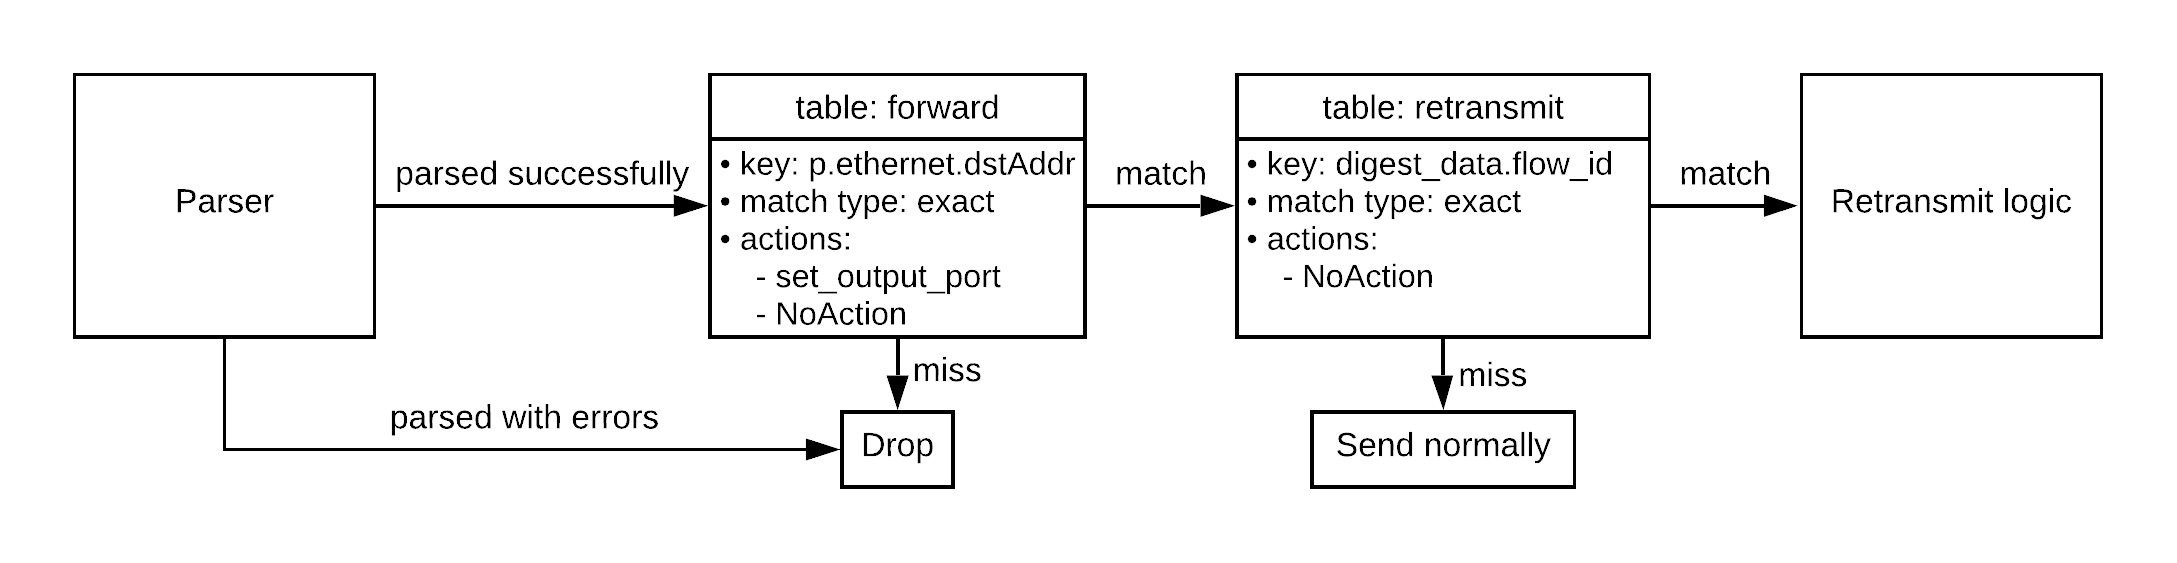
\includegraphics[width=\textwidth]{mapipe.png}
	\caption{A packet processing program describing a simple L2/L3 IPv4 switch.}
	\label{mapipe}
\end{figure}

When we defines a match-action table (using the P4 \textbf{\texttt{table}} keyword), we declare various properties such as the header and/or metadata field(s) to match upon, the type of match to be performed, a list of all possible actions that can be invoked, the number of entries to allocate for the table, and a default action to invoke if no match is found. A table entry contains a specific key to match on, a single action to invoke when the entry produces a match, and any data to provide to the action when it is invoked. Table entries are populated at runtime by the control plane software.

\begin{table}[!h]
	\centering
	\caption{Entries for the \texttt{forward} table.}
	\label{forward}
	\begin{tabular}{ | c | c | c |}
		\hline
		\textbf{Key} & \textbf{Action} & \textbf{Action Data} \\ \hline
		08:11:11:11:11:08 & \verb|set_output_port| & 0b00000001 \\ \hline
		08:22:22:22:22:08 & \verb|set_output_port| & 0b00000100 \\ \hline
		08:33:33:33:33:08 & \verb|set_output_port| & 0b00010000 \\ \hline
		08:44:44:44:44:08 & \verb|set_output_port| & 0b01000000 \\ \hline
		ff:ff:ff:ff:ff:ff & \verb|set_output_port| & 0b01010101 \\ \hline
	\end{tabular}
\vspace{2em}
	\centering
	\caption{Entries for the \texttt{retransmit} table.}
	\label{retransmit}
	\begin{tabular}{ | c | c | c |}
		\hline
		\textbf{Key} & \textbf{Action} & \textbf{Action Data} \\ \hline
		\texttt{792281630049477301766976897099}  & NoAction & \_ \\ \hline
	\end{tabular}
\end{table}

Figure \ref{mapipe} illustrates the control flow program acting on a packet going through our match-action pipeline, which comprises two match-action tables: \texttt{forward} and \texttt{retransmit}.
The first table uses the Ethernet destination address to determine the output port for the next hop. If this lookup fails, the packet is dropped (by assigning \texttt{sume\_metadata.dst\_port} to 0). The second table checks the computed \texttt{digest\_data.flow\_id}: if it matches our flow of interest, the packet will be monitored to assist the fast retransmit of TCP congestion control. Otherwise, the packet will just be sent normally. A packet will be modified by a series of \texttt{action}s: \texttt{set\_output\_port} sets the output port on the SUME board for packets whose Ethernet destination address matches what was defined in the first table, and \texttt{compute\_flow\_id} computes the flow number of the packet for the second table to look up. \texttt{cache\_write}, \texttt{cache\_read} and \texttt{cache\_drop} modify \texttt{digest\_data.tuser} to signal the cache queue to cache, retransmit and drop the packet at the head of the queue respectively.

In summary, the switch will perform the following tasks in the SSS module:
\begin{itemize}
	\item Receive and parse packet from the sender.
	\item Look up the Ethernet destination address to determine the output port. Drop on a miss.
	\item Compute the flow number of the packet.
	\item Look up the flow number of the packet to determine if it should be monitored. Send normally on a miss.
	\item Set \texttt{digest\_data.tuser} and/or set the \texttt{ACK} flag in the TCP header appropriately.
	\item Construct the final packet and send it to the receiver.
\end{itemize}

	\subsection{The Extern Functions}
P4 extern functions, or externs, are platform-specific functions that are not described in the core P4 language---a kind of ``black boxes'' for P4 programs. Extern functions are implemented in HDL and the P4 program just sees the inputs and outputs, as parameters and results. There are two types of extern functions: stateless (reinitialised for each packet) and stateful (keeping states between packets). The stateful atomic externs are inspired by the Domino atoms \cite{domino}. P4$\rightarrow$NetFPGA provides a set of commonly-used extern functions, shown in Table \ref{externs}, in the \texttt{templates} folder. 

\begin{table}[!ht]
	\begin{center}
		\caption{The P4$\rightarrow$NetFPGA extern functions library.}
		\label{externs}
		\begin{tabular}{ | c | c | }
			\hline
			\multicolumn{2}{|c|}{\textbf{Stateful Atomic Extern Functions}} \\ \hline
			\textbf{Name} & \textbf{Description}  \\ \hline
			RW & Read or write state \\ \hline
			RAW & Read, add to, or overwrite state  \\ \hline
			PRAW & Either perform RAW or do not perform RAW based on predicate \\ \hline
			ifElseRAW & Two RAWs, one each for when a predicate is true or false \\ \hline
			Sub & IfElseRAW with stateful subtraction capability \\ \hline
			
			\multicolumn{2}{|c|}{\textbf{Stateless Extern Functions}} \\ \hline
			\textbf{Name} & \textbf{Description}  \\ \hline
			IP Checksum & Given an IP header, compute the IP checksum \\ \hline
			LRC & Longitudinal redundancy check, simple hash function \\ \hline
			timestamp & Generate timestamp (measured in clock cycles, granularity of 5ns) \\ \hline
		\end{tabular}
	\end{center}
\end{table}

An extern function can be declared using the syntax

{\renewcommand{\baselinestretch}{0.8}\small
	\centering
	\begin{verbatim}
 extern void <name>_<extern_type>(in T1 data1,in T2 data2,...,out D result);
	\end{verbatim}
} 

The following code sequence shows an example of declaring a simple longitudinal redundancy check hash extern:

{\renewcommand{\baselinestretch}{0.8}\small
	\begin{verbatim}
    @Xilinx_MaxLatency(1)
    @Xilinx_ControlWidth(0)
    extern void hash_lrc(in T in_data, out D result);
	\end{verbatim}
}
where \texttt{@Xilinx\_MaxLatency} and \texttt{@Xilinx\_ControlWidth} are Xilinx P4-SDNet's additional annotations to allow P4 programmer to specify the number of clock cycles to complete the extern operation, and the width of the address space allocated to this register respectively. The control width should always be equal to the width of the index field so that the control plane can access all register entries.

For this design, I defined the following externs using the available extern functions provided by P4$\rightarrow$NetFPGA:
\begin{itemize}
	\item \verb|hash_lrc|: a simple hash function that splits the input data into multiple words and \textit{XOR} each word together to obtain the result. The hash result is used to index into the registers.
	\item \verb|seq_no_reg_praw|: stores the latest sequence number from the sender. This is updated when a new packet is received from the sender.
	\item \verb|latest_ack_no_reg_praw|: stores the latest acknowledgement number from the receiver. This is updated when a new ACK packet is received from the receiver. 
	\item \verb|pkts_cached_cnt_reg_raw|: stores the number of packets that the cache queue is buffering. This is updated when a new packet is buffered to, or when some packets are dropped or read from the cache queue.
	\item \verb|ack_cnt_reg_praw|: stores the number of duplicate acknowledgements. This is updated when the switch received a duplicate acknowledgement, that is \verb|p.tcp.ackNo == latest_ack_no|. When the value of the counter reaches 2, the third duplicate acknowledgement will trigger the retransmission.
	\item \verb|retransmit_cnt_reg_ifElseRaw|: stores the number of retransmission of the DUP ACK packet. Once a retransmission occurs, this counter will be set to 1. Subsequent DUP ACK packet will be sent back to the sender since the switch would now assume that the reason for packet loss is due to packet corruption.
\end{itemize}

An important feature of P4$\rightarrow$NetFPGA externs is that to guarantee consistency between successive packets, stateful operations cannot be pipelined; each performs an atomic read-modify-write operation per packet. In other words, each stateful atom can only be accessed \textit{one} time in the P4 code. Multiple calls to the extern function will generate multiple instances of the atom, thus giving unexpected results. This complicates my design since intuitively, we would usually require two operations to perform the logic. For instance, one needs to first perform a \textit{read} operation from the register to get the latest sequence number stored to determine if this packet is a new packet. If it is indeed a new packet, one then needs to perform a ``write'' operation to update the value of the latest sequence number stored.

	\subsection{The Deparser}
The inverse of parsing is deparsing, or packet assembly, where the outgoing packet is constructed by reassembling the packet headers as computed by the pipeline onto an outgoing packet byte stream. P4 does not provide a separate language for packet deparsing; deparsing is done in a \textbf{\texttt{control}} block that has at least one parameter of type \verb|packet_out| because it only involves sequential logic as used for actions. The advantage of this approach is that it makes deparsing explicit, but decouples it from parsing. 

A header is added to the packet using the \verb|packet_out| object's \texttt{emit} method. following code block, which implements the deparser of the switch, first writes an Ethernet header, followed by an IPv4 header, and then a TCP header into a \verb|packet_out|. Since emitting a header appends the header to the \verb|packet_out| only if the header is valid, P4 first checks the validity of the headers before serialising them.

{\renewcommand{\baselinestretch}{0.8}\small
\begin{verbatim}
  // Deparser Implementation
  @Xilinx_MaxPacketRegion(8192)
  control TopDeparser(packet_out b,
                  in Parsed_packet p,
                  in user_metadata_t user_metadata,
                  inout digest_data_t digest_data, 
                  inout sume_metadata_t sume_metadata) { 
      apply {
        b.emit(p.ethernet); 
        b.emit(p.ip);
        b.emit(p.tcp);
      }
  }
\end{verbatim}
}

\section{Hardware Implementation}
	\label{sec:cachequeue}
	\subsection{The Cache Queue}
The cache queue has the basic functionalities similar to those of the output queue of the NetFPGA reference switch design (see Figure \ref{fig:netfpga-ref-switch}): buffer packets from the SimpleSumeSwitch module while they wait to be sent to the output ports. However, since the role of the cache queue is to buffer packets to \textit{retransmit}, we want to be able to signal to the cache queue when to buffer a packet, when to drop a packet, when to read a packet and how many packets to drop. This is done by using the metadata of the packet. More specifically, recall from section \ref{sec:p4-netfpga} that the P4 programmer can define the format of the \verb|digest_data| bus. The only constraint is that it \textit{must} be defined to be 256 bits wide. Thus, to implement the signalling functiont to the cache queue, it is configured it as follows:

{\renewcommand{\baselinestretch}{0.8}\small
	\begin{verbatim}
    struct digest_data_t {
      bit<72>  unused;
      bit<104> flow_id;
      bit<80> tuser;
    }
	\end{verbatim}
}

The \verb|digest_data| bus is then trimmed to the first 80 bits, and together with the \verb|sume_metadata| bus form the \texttt{tuser} signal. The format of the \texttt{tuser} signal and the \texttt{digest\_data} field are shown in Table \ref{tab:tuser} and \ref{tab:digest-data}.

\begin{table}[!h]
	\centering
	\caption{Format of the \texttt{tuser} signal.}
	\label{tab:tuser}
	\begin{tabular}{ | c | c | >{\centering\arraybackslash}m{9.5cm} |}
		\hline
		\textbf{Bits} & \textbf{Name} & \textbf{Comments} \\ \hline
		[15:0] & \verb|pkt_len| & Unsigned \verb|int| \\ \hline
		[23:16] & \verb|src_port| & One-hot encoded: \{DMA, NF3, DMA, NF2, DMA, NF1, DMA, NF0\} \\ \hline
		[31:24] & \verb|dst_port| & One-hot encoded: \{DMA, NF3, DMA, NF2, DMA, NF1, DMA, NF0\} \\ \hline
		[39:32] & \verb|drop| & Only bit 32 is used \\ \hline
		[47:40] & \verb|send_dig_to_cpu| & Only bit 40 is used \\ \hline
		[127:48] & \verb|digest_data| & The first 80 bit of the \verb|digest_data| bus from the SimpleSumeSwitch module \\ \hline
	\end{tabular}
	\vspace{1em}
	\centering
	\caption{Format of the \texttt{digest\_data} field.}
	\label{tab:digest-data}
	\begin{tabular}{ | c | c | c |}
		\hline
		\textbf{Bits} & \textbf{Name} & \textbf{Comments} \\ \hline
		[55:48] & \verb|cache_write| & Encoded: \{0, 0, 0, DMA, NF3, NF2, NF1, NF0\} \\ \hline
		[63:56] & \verb|cache_read| & Encoded: \{0, 0, 0, DMA, NF3, NF2, NF1, NF0\} \\ \hline
		[71:64] & \verb|cache_drop| & Encoded: \{0, 0, 0, DMA, NF3, NF2, NF1, NF0\} \\ \hline
		[79:72] & \verb|cache_count| & Number of packets to read or drop \\ \hline
		[127:80] & unused & - \\ \hline
	\end{tabular}
\end{table}

NOTE: where should I explain what the \texttt{tuser} signal is? Also, should I explain the whole input and output, master and slave to each of the module and where should I explain that (if necessary)? And also the AXI components?

	\subsection{The Output Arbiter}
The NetFPGA reference switch design also comes with an input arbiter (see Figure \ref{fig:netfpga-ref-switch}) whose function is to merge multiple input streams into one output stream. All input interfaces share the same bandwidth (and therefore width) as the output stream to ensure that maximum throughput can be achieved. For our architecture (see Figure \ref{fig:modified-design}), since we have two queues---the output queue and the cache queue---we would require an ``output'' arbiter for each of the five output ports. 

The only difference between the output arbiter and the input arbiter is the number of input streams: the input arbiter has 5 input streams from 5 RX queues while the output arbiter has only 2 input streams from the output queue and the cache queue. Thus, I simply duplicated the implementation of the input arbiter in the NetFPGA reference switch design and removed the extra 3 slave stream ports and changed the appropriate variables and wires to match the number of input streams.

NOTE: Is this sufficient? I think that was all I did for the output arbiter.

	\subsection{The Reference Switch Design}

The \verb|nf_datapath.v| Verilog file describes the hardware structure of the reference switch design. It specifies the logical circuit of the design that allows for the automated analysis and simulation. I modified the NetFPGA reference switch design by adding the cache queue and the output arbiter HDL modules and wiring the inputs and outputs of each module accordingly. The wiring process is tedious, due to the large number of inputs and outputs of each module.
	
	\subsection{IP Core Generation}
IP cores are stand-alone HDL modules. They are configurable and reusable.

NOTE: I am not sure what to write here.
	\subsection{Project Wrappers}
NOTE: I am not sure what to write here.


